\begin{frame}[Core Problem ]
\frametitle{Introduction}
\begin{itemize}
\item \small Noise Amplification Problem(NAP) is a fundamental inhibitor for bulk-synchronous MPI applications running at very large scale.
\item \small Several scientific simulations at LLNL are bulk-synchronous in nature, and thus suffer the noise amplification problem.
\item \small We believe that through our lightweight scheduling approaches, you can scale past this noise amplification problem at large scales.
\item \small We hope that you will be convinced to use our techniques in your codes.
\end{itemize}
\end{frame}


\begin{frame}
\frametitle{Noise Amplification Problem(NAP)}

\begin{itemize}
\item NAP causes 28\% degradations on Jaguar at maximum scale.
\item NAP cause 37\% degradations on Ranger at maximum scale.
\item Through simulation of exascale machines, these numbers shoot up to 47\% and 53\% on Jaguar and Ranger respectively.
\end{itemize}
\end{frame}

\begin{frame}
\frametitle{Lightweight Scheduling Techniques}
\begin{itemize}
\item Tasklet Granularity Scheduling: Adapts for probabilistic noise.
\item Weighted Dynamic Scheduling: Adapts for periodical noise.
\item Slack-conscious Lightweight Scheduling: reduces scheduling on those MPI processes not on critical path.
\end{itemize}
\end{frame}

\begin{frame}
\begin{columns}
\column{0.5\textwidth}
\begin{enumerate}
\item \tiny Tasklet grainularity $\mu$-scheduling noticiably reduces noise amplification on both machines, and gives a large 55\% performance gain.
\item \tiny Weighted $\mu$-scheduling provides noticeable(above 30\%) gains on
  both machines,  due to this scheduler's ability to handle any mixture
  of low-prob, high-amp load imbalance and high-freq, low-amp load
  imbalance.
\item \tiny Slack-conscious lightweight scheduling provides 25\% performance gains on both machines.
\end{enumerate}
\column{0.5\textwidth}
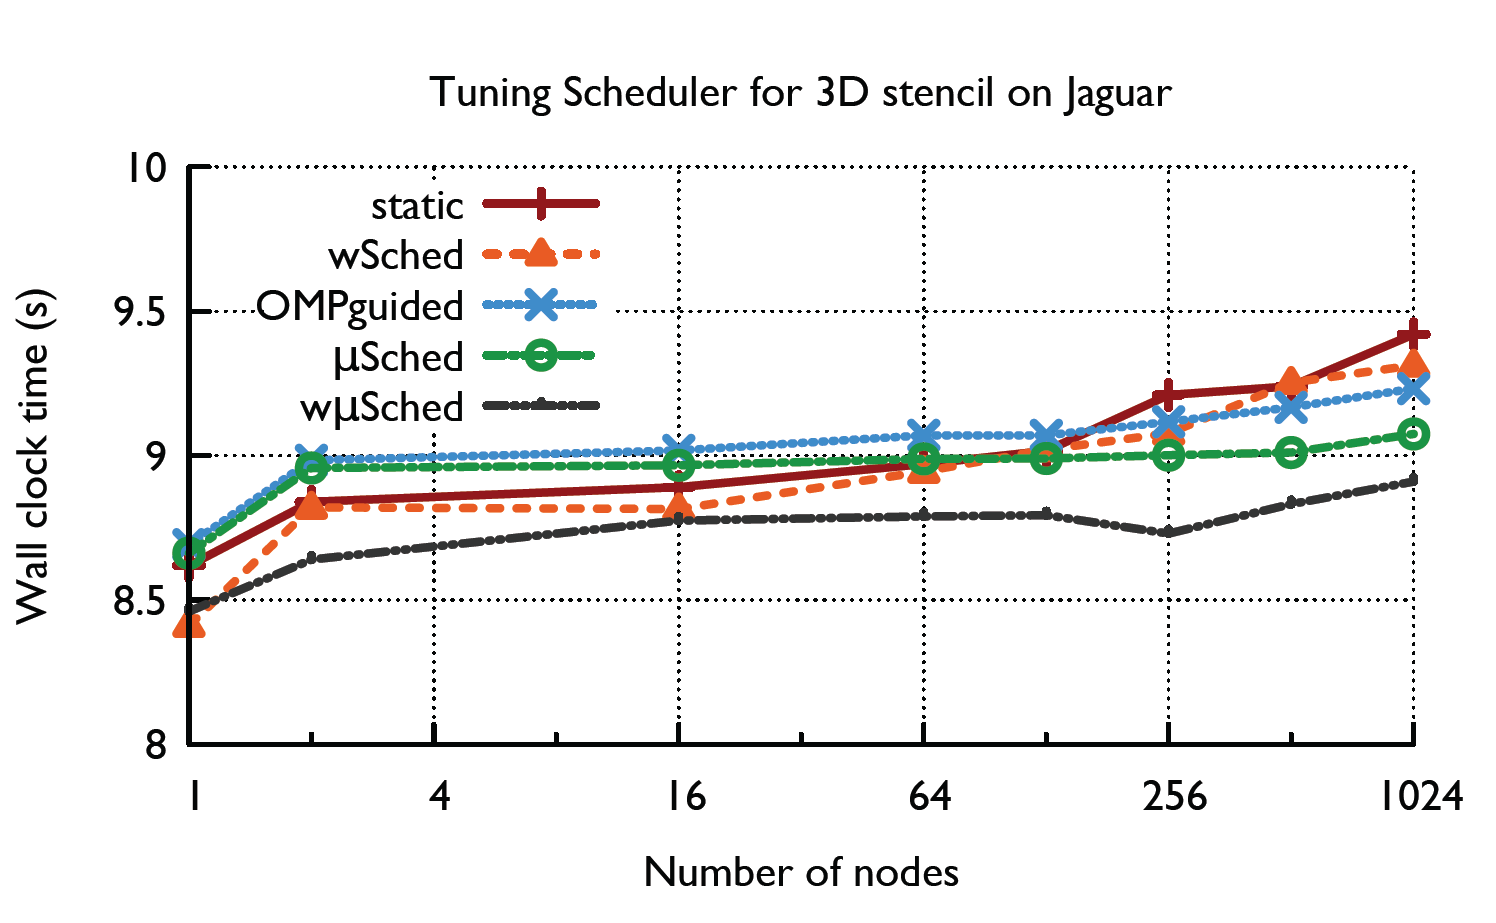
\includegraphics[width=\textwidth]{images/schedulerTuningJaguar} \\
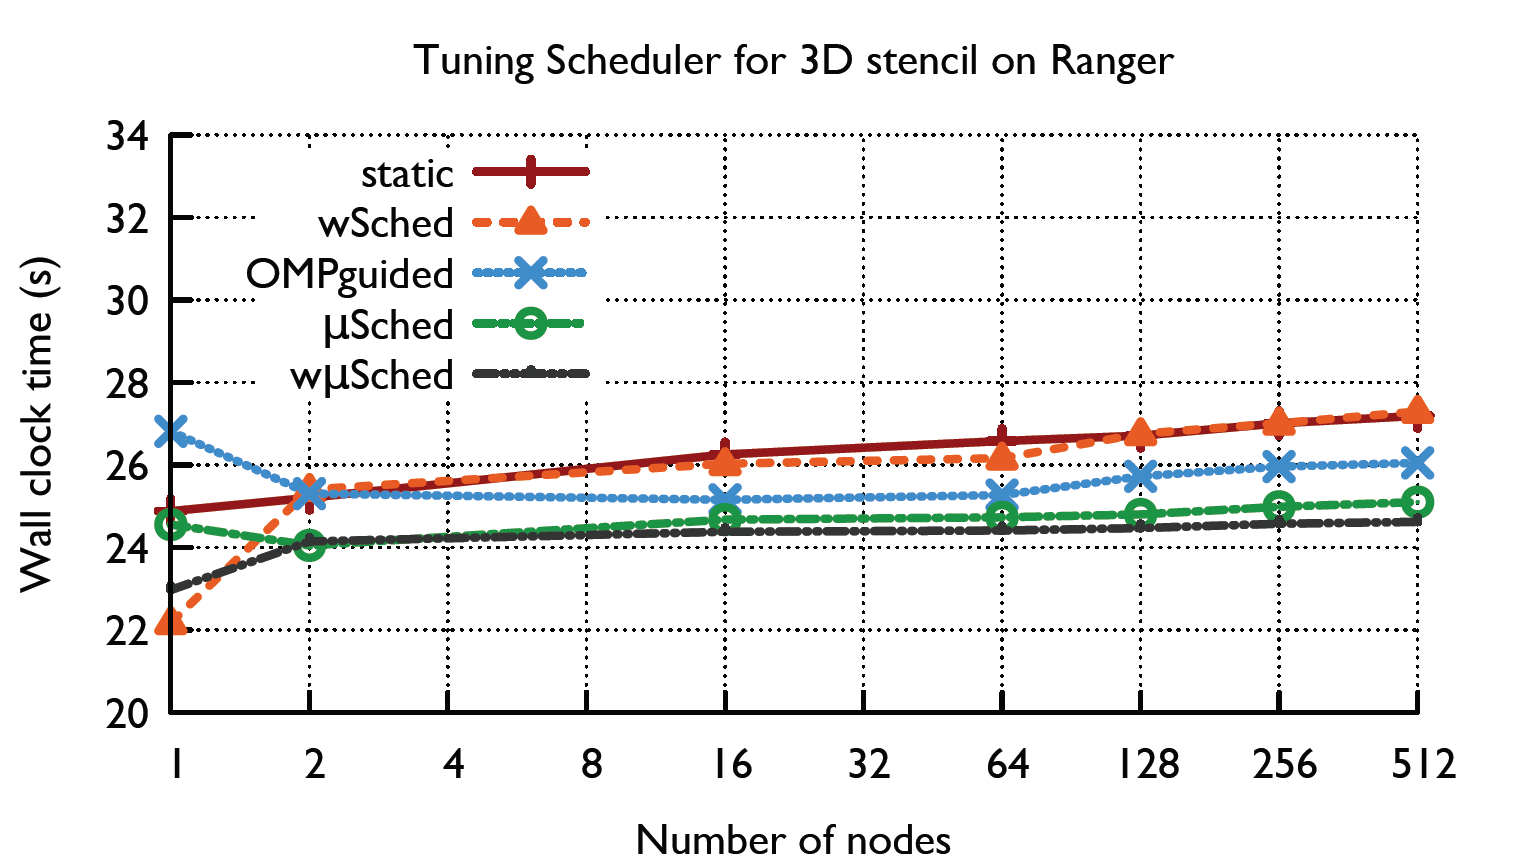
\includegraphics[width=\textwidth]{images/schedulerTuningRanger}
\end{columns}
\end{frame}

\begin{frame}
\frametitle{Conclusions}
\begin{itemize}
\item Several scientific codes at the lab are bulk-synchronous in nature, and thus will suffer the noise amplification problem.
\item We get significant (up to 55\%) performance gains using our techniques,  in the presence of NAP.
\item Using our techniques, you will be able to do more science per hour.
\item You can obtain our software at www.blahblahblah.com. We hope that you will consider it before your next large-scale application run!
\end{itemize}
\end{frame}


